%%%% fatec-article.tex, 2024/03/10

%% Classe de documento
\documentclass[
  a4paper,%% Tamanho de papel: a4paper, letterpaper (^), etc.
  12pt,%% Tamanho de fonte: 10pt (^), 11pt, 12pt, etc.
  english,%% Idioma secundário (penúltimo) (>)
  brazilian,%% Idioma primário (último) (>)
]{article}

%% Pacotes utilizados
\usepackage[]{fatec-article}
\usepackage{float} % ← ADICIONE ESTE PACOTE
\Author{1}{Name={Araujo, A\\ Santos, E \\ Sueoka, L \\ Estevam, R }}

\Author{2}{Name={\{ andrei.araujo01@fatec.sp.gov.br \}\\ \{ erlon.santos3@fatec.sp.gov.br \} \\ \{ leandro.sueoka@fatec.sp.gov.br \} \\ \{ ricardo.conceicao@fatec.sp.gov.br \} }}

%% Definição das palavras-chaves/keywords
\Keyword{1}{Fazendas verticais}{Vertical farms}
\Keyword{2}{Inteligencia artificial}{Artificial intelligence}
\Keyword{3}{ODS}{SDG}

%%%% Resumo no idioma primário (brazilian)
\begin{Abstract}[brazilian]%% Idioma (brazilian ou english)
  Fome, indústria, inovação e agricultura sustentável são alguns dos desafios mundiais apontados pela Organização das Nações Unidas. Neste âmbito as fazendas verticais são uma alternativa promissora por fornecerem alta produtividade em áreas reduzidas e utilizando poucos recursos. Além disso, para que possam operar de forma autônoma, necessitam de tecnologias como internet das coisas e inteligência artificial. Com base nisso, este trabalho propõe-se a desenvolver e validar uma Arquitetura de Gerenciamento de Fazendas Verticais controladas por Inteligência Artificial. O sistema utiliza uma rede de sensores IoT para coletar dados críticos (fluxo hídrico e concentração de nutrientes), os quais são transmitidos e processados em um servidor cloud. A IA centraliza a análise destas informações, emitindo ajustes prescritivos e automáticos para o ambiente de cultivo.
\end{Abstract}

%%%% Resumo no idioma secundário (english)
\begin{Abstract}[english]%% Idioma (brazilian ou english)
  Hunger, industry, innovation, and sustainable agriculture are some of the global challenges identified by the United Nations. In this context, vertical farms represent a promising alternative, as they provide high productivity in limited areas while using few resources. Furthermore, to operate autonomously, they require technologies such as the Internet of Things and Artificial Intelligence. Based on this, this work proposes the development and validation of an AI-Controlled Vertical Farm Management Architecture. The system uses an IoT sensor network to collect critical data (water flow and nutrient concentration), which is transmitted and processed on a cloud server. The AI centralizes the analysis of this information, issuing prescriptive and automatic adjustments for the cultivation environment.
\end{Abstract}

%% Processamento de entradas (itens) do índice remissivo (makeindex)
\makeindex%

%% Arquivo(s) de referências
\addbibresource{fatec-article.bib}

%% Início do documento
\begin{document}

% Seções e subseções
%\section{Título de Seção Primária}%

%\subsection{Título de Seção Secundária}%

%\subsubsection{Título de Seção Terciária}%

%\paragraph{Título de seção quaternária}%

%\subparagraph{Título de seção quinária}%

\section*{Introdução}%
\label{sect:intro}
A ONU (Organização das Nações Unidas) e seus parceiros trabalham para atingir os 17 Objetivos de Desenvolvimento Sustentável (ODS) que abordam os principais desafios enfrentados no Brasil e no mundo \cite{nacoesunidas2024}. Os objetivos envolvem ações para combater a pobreza, proteger o clima e meio ambiente, e garantir paz e prosperidade às pessoas. As ODS 2, ODS 9, ODS 11 e ODS 12 tratam, respectivamente, de fome zero e agricultura sustentável, indústria, inovação e infraestrutura, cidades e comunidades sustentáveis e consumo e produção responsáveis, objetivos que convergem diretamente com o agronegócio.

Atualmente o agronegócio no Mercado Comum do Sul (Mercosul, composto por Argentina, Brasil, Paraguai, Uruguai, Venezuela e Bolívia) é responsável por aproximadamente 10\% das exportações mundiais, sendo o principal exportador de commodities agrícolas básicas \cite{agenciagov2024}. O agronegócio brasileiro representa 22,3\% do PIB (Produto Interno Bruto) em 2024, sendo uma das principais forças econômicas do país \cite{cepea2024}.

O Produto Interno Bruto (PIB) do Estado de São Paulo fechou o ano de 2024 em R\$ 3,5 Tri \cite{agenciasp2025}, representando cerca de 30\% do PIB brasileiro \cite{desiderio2024}. Deste montante, o valor proveniente do PIB da cidade de São Paulo é de 1,12 Tri, ou seja, 32\% do estado \cite{seade2025}. A divisão do PIB municipal mostra que 7,5\% do montante é proveniente da indústria, 20,3\% são impostos líquidos e 72,2\% pertencem ao setor de serviços, não havendo participação do agronegócio \cite{seade2025}. No setor de serviços, destaca-se a quantidade de estabelecimentos voltados à alimentação fora do lar, como padarias, restaurantes e lanchonetes, com 144,9 mil estabelecimentos \cite{sindresbar2024}.

A cidade de São Paulo possui 11,9 milhões de habitantes \cite{agenciabrasil2025}, dos quais 5,8 milhões enfrentam alguma situação de insegurança alimentar \cite{radioagencia2024}. Em contrapartida, estão mapeadas apenas 818 Unidades de Produção Agropecuária e 209 hortas urbanas \cite{sampa2025}.

Fazenda vertical é um conceito criado por Despommier (1999) e vem se aperfeiçoando ao longo dos anos. Consiste em um modelo de cultivo em locais fechados e ambiente controlado, combinado com técnicas como a hidroponia. No Brasil, há mais de 20 fazendas verticais, número baixo em comparação com os EUA, que possuem cerca de 2 mil plantações deste tipo \cite{costa2025}. Para São Paulo, é um modelo aplicável, podendo ampliar a produção em até 30 vezes em um tempo 70\% menor comparado aos modelos tradicionais \cite{gundim2022}.

O cultivo em fazendas verticais apresenta vantagens como ausência de secas, alagamentos e granizo, melhor controle de pragas, economia de água graças ao reuso e não degradação do solo \cite{ingram2023}. É um modelo escalável, podendo ser aplicado desde pequenos espaços até arranha-céus, controlando luz, ambiente, umidade, temperatura, gases e fertirrigação \cite{lucena2021}.

A hidroponia, embora ainda não tão difundida no Brasil, cresce continuamente. Proporciona controle de nutrientes, antecipação da colheita, padronização da quantidade e qualidade, menor incidência de pragas e racionalização da energia. Sua desvantagem é a necessidade de acompanhamento constante do sistema produtivo \cite{luz2006}. A alface (Lactuca sativa L.), especialmente o grupo Solta-Crespa, é uma das hortaliças mais importantes, representando 70\% do mercado brasileiro. Combinada com a hidroponia, o tempo de colheita é reduzido em cerca de 10 dias \cite{luz2006}.

A tecnologia IoT (Internet das Coisas) permite conectar objetos inteligentes à internet, transmitindo dados de forma segura \cite{carnaz2016}. Combinada com redes neurais, é útil para monitoramento contínuo em fazendas verticais. O aprendizado de máquina (Machine Learning) é um ramo da IA que constrói sistemas capazes de aprender a partir de dados e gerar modelos de predição ou classificação \cite{paixao2022}. Redes neurais são sistemas compostos por unidades de processamento simples, semelhantes ao funcionamento do cérebro humano \cite{haykin2001}. Entre elas, as redes neurais recorrentes (RNN) tratam dados sequenciais, sendo úteis para reconhecimento de padrões, tradução de textos e predição de valores de mercado \cite{baronte2022}.

Agricultura 4.0 é baseada na aplicação de tecnologias como IoT, robótica, sensores, IA e aprendizado de máquina, visando produtividade, lucratividade e ecoeficiência \cite{lisbinski2020}. Alinhado a esse conceito, temos as Smart Farms, que são fazendas inteligentes equipadas com IoT e conhecimento especializado, permitindo cultivo até por pessoas com pouca experiência e oferecendo vantagens como prevenção e detecção de doenças \cite{ryu2015}.

Na literatura, existem propostas combinando Fazendas Verticais e IoT, com dados utilizados por RNN, permitindo resultados distintos daqueles observados em métodos tradicionais.

\section*{OBJETIVO} \label{sect:obj}

O objetivo principal deste projeto é desenvolver uma proposta de ambiente autônomo para gerenciamento de fazendas verticais. O gerenciamento será realizado por meio de uma aplicação web, com o monitoramento e controle de concentração de fertilizantes e do fluxo de água utilizada.

Objetivos específicos: desenvolvimento de uma proposta sustentável, economicamente viável e que incorpore novas tecnologias ao modelo de cultivo presente na região; viabilizar uma proposta que melhore a produtividade ao passo que utilize menos recursos que o modelo tradicional de produção.

\section*{ESTADO DA ARTE} \label{sect:estadoarte}

O objeto de estudo deste projeto são fazendas verticais e o uso de tecnologia. Realizando busca por artigos neste sentido, foram identificados alguns trabalhos com a mesma temática. Saraswathy et al. \cite{saraswathy2020} apresentaram um trabalho muito parecido com o nosso, relatando a integração de inteligência artificial utilizando IoT em uma fazenda hidropônica focada no estado de Tamil Nadu, no sul da Índia. A proposta monitorava parâmetros de umidade, pH, temperatura, intensidade de luz e fluxo de água por meio de sensores, enviando os valores para a nuvem via Node MCU. Utilizando uma rede neural recorrente (RNN) do tipo Long-Short-Term Memory (LSTM) com algoritmo de previsão visando maior precisão na automação, o trabalho apresentou resultados satisfatórios, eliminando a necessidade de acompanhamento constante pelos fazendeiros e permitindo que os erros apresentados pela rede neural fossem utilizados para automatizar toda a produção da fazenda hidropônica. Este trabalho se assemelha ao nosso pelo uso de redes neurais em um ambiente de fazenda vertical, embora não utilize aplicação móvel e monitore mais parâmetros do que os planejados neste estudo.

Souza \citeyear{sousa2023} desenvolveu um projeto sobre um sistema baseado em IoT e sensores para supervisão e controle de fazendas verticais. O projeto foi constituído de um módulo gerenciado por microcontrolador, estufa e banco de dados hospedado em um computador pessoal. O módulo dispunha de entradas e saídas analógicas e digitais (para conexão dos sensores utilizados), além de conexão sem-fio. O autor relatou que os objetivos propostos foram alcançados, utilizando um equipamento de custo acessível e monitoramento constante. O trabalho se assemelha à nossa proposta pelo uso de fazendas verticais e IoT, porém diverge por não utilizar nenhum sistema de inteligência artificial, tratando os dados coletados apenas dentro de intervalos para tomada de decisão.

Rakhmatulin \cite{rakhmatulin2021} apresentou um sistema automatizado combinando IoT e rede neural, juntamente com um software desenvolvido pelo autor, câmera digital e sensores de luminosidade, gás carbônico, temperatura, umidade, ph e temperatura do solo. Em sua proposta o autor se utilizou de um ambiente fechado em que 7 sensores monitoram o crescimento da hortaliça. Por sua vez o sinal dos sensores é encaminhado para um controlador que envia os dados para uma rede neural avaliar e fazer a gestão do cultivo. Este sistema difere da nossa proposta por empregar agricultura convencional e ter foco no cultivo de tomates.

Ahmareen et al. \cite{ahmareen2024} apresentaram um sistema utilizando IoT para gerenciar uma fazenda vertical. Combinado com tecnologias para monitoramento remoto, sensores e bancos de dados, o sistema buscava melhorar a gestão da fazenda vertical e desenvolver um modelo de custo acessível. A metodologia utilizada combinava sensores de umidade, chuva, solo e temperatura com um controlador que, por sua vez, encaminhava os dados para a nuvem. Estes dados eram convertidos em gráficos e apresentados em uma tela, tornando possível a tomada de decisão no controle de uma bomba d’água e sistema de ventilação. Embora os objetivos tenham sido alcançados, o autor encontrou dificuldades com os custos de instalação e manutenção do sistema IoT, além da instabilidade da internet em algumas localidades. Diferentemente do nosso trabalho, não foi utilizado nenhum sistema de rede neural para gerenciamento automático.


\section*{METODOLOGIA} \label{sect:metodologia}

Para a problemática de uma fazenda vertical autônoma orientada por redes neurais foi definida uma metodologia baseada no ciclo Planejar-Fazer-Verificar-Agir (do inglês, Plan-Do-Check-Act ou PDCA) e consiste em a) revisão bibliográfica; b) planejamento da solução lógica do sistema; c) definição das tecnologias, layout do sistema e funcionalidades e d) prototipação.
\begin{figure}[H]
    \centering
    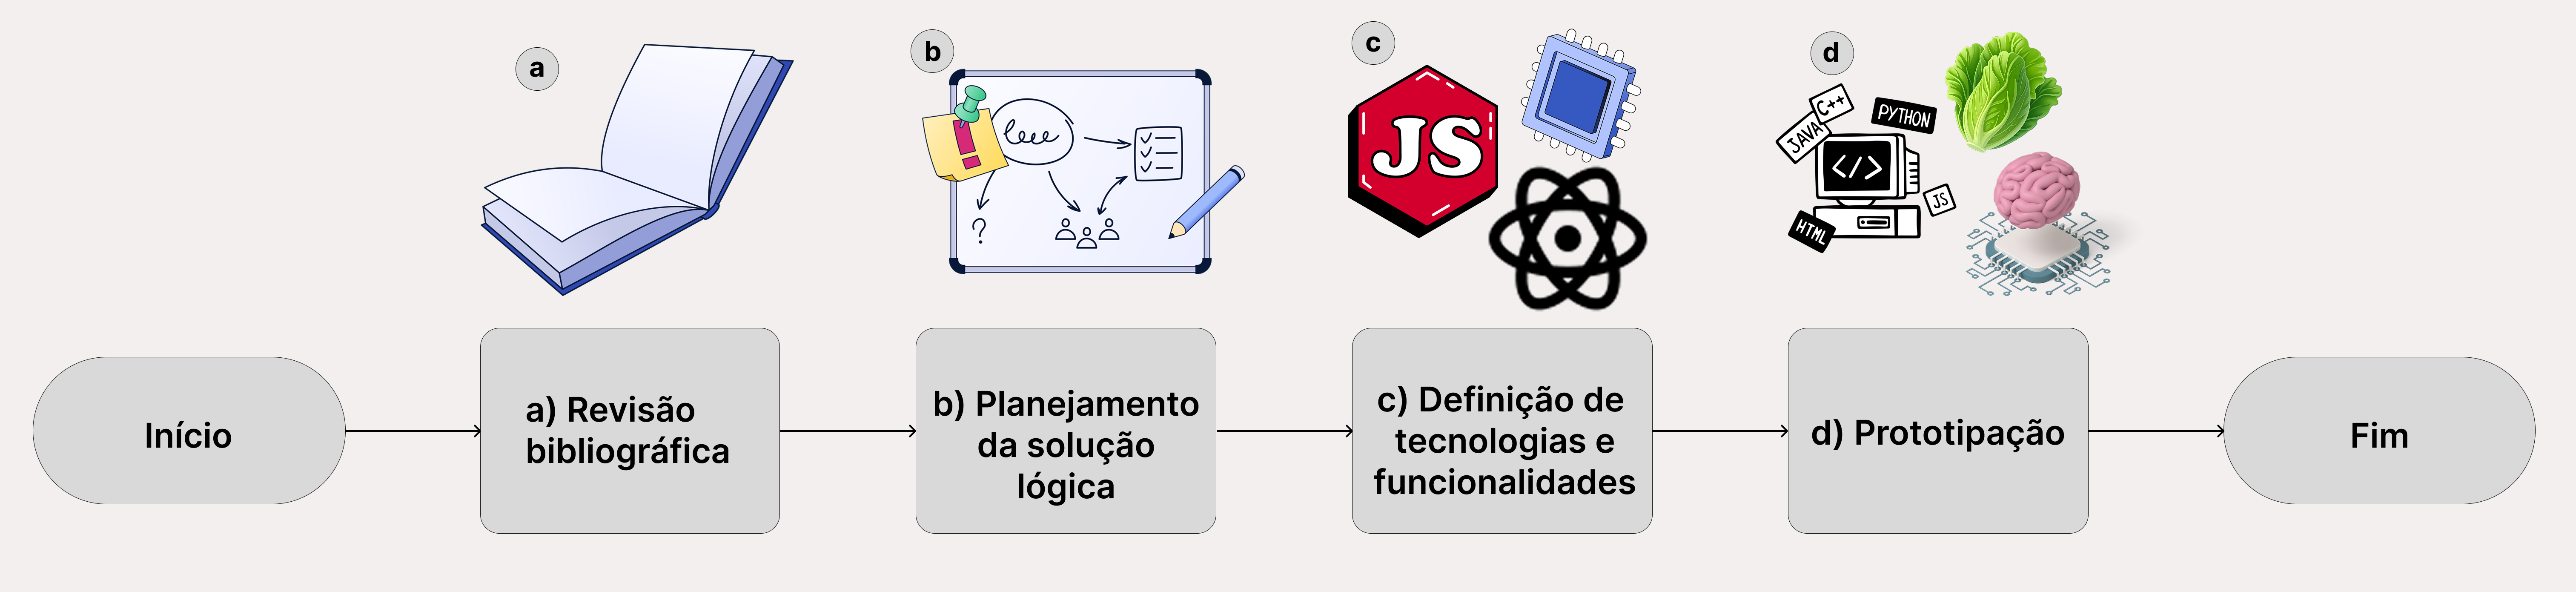
\includegraphics[scale=0.08]{Illustrations/Figura 1.png} % sem extensão se for .png
    \caption{Metodologia adotada para o desenvolvimento do sistema de fazenda vertical autônoma com redes neurais, organizada em quatro etapas sequenciais.
}
    \label{fcht:figura1}
    % \SourceOrNote{Autoria Própria (2024)} % só se esse comando estiver definido
\end{figure}

Após a etapa a) verificação da literatura existente (Estado da Arte), a etapa b) planejamento indicou duas possibilidades: na Figura 2 a fazenda vertical (1) envia, por meio de sensores IoT de nível de água, os dados atuais de fluxo de água e fertilização para um banco de dados na nuvem (2). Estes dados podem ser acessados pelo cliente, por meio de software, onde o usuário pode diretamente tomar a decisão de como devem operar o fluxo de água e fertilização da fazenda, recomeçando o ciclo.


\begin{figure}[H]
    \centering
    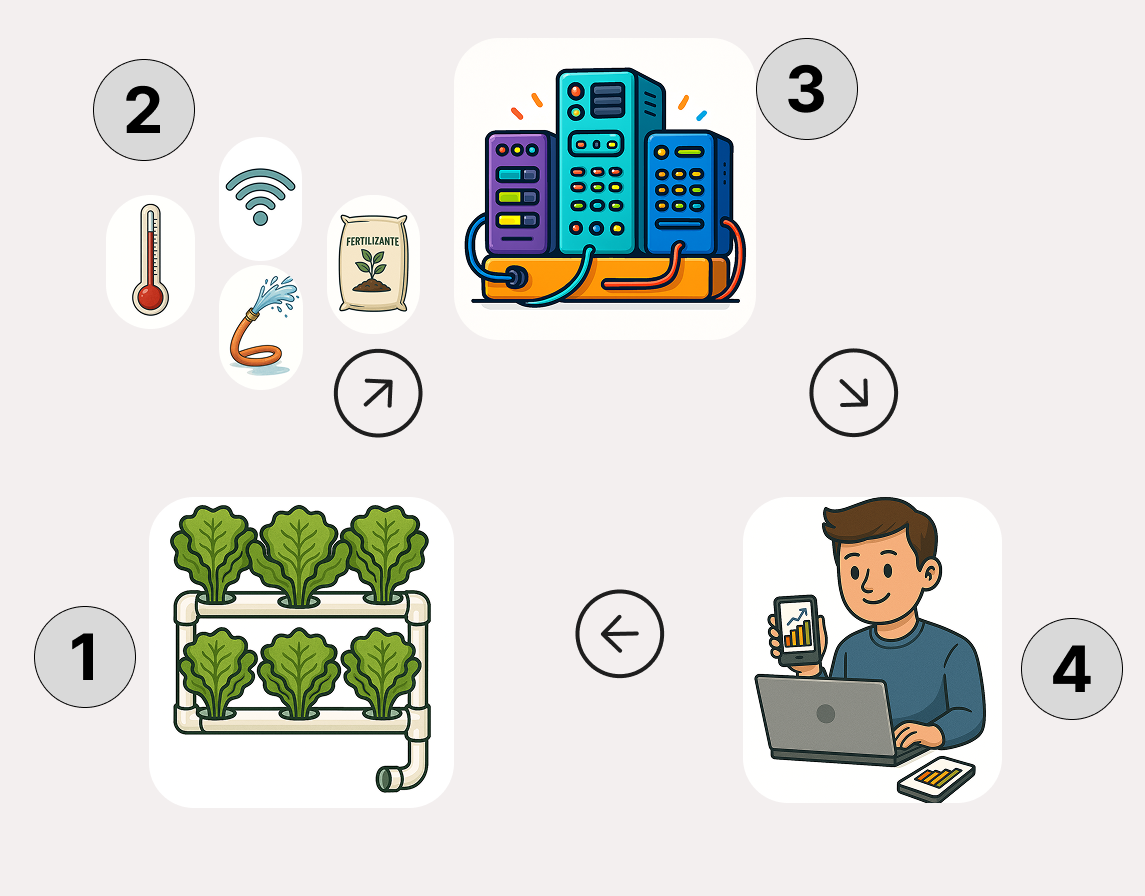
\includegraphics[scale=0.2]{Illustrations/Figura 2.png} % sem extensão se for .png
    \caption{Exemplo de funcionamento do sistema proposto utilizando 4 etapas, mantendo a tomada de decisão sob controle do usuário.}
    \label{fcht:figura2}
    % \SourceOrNote{Autoria Própria (2024)} % só se esse comando estiver definido
\end{figure}


Também é possível que a fazenda vertical (1) envie os dados de fertilizantes e fluxo de água (2) para um banco de dados na nuvem (3). Porém quem faz a avaliação e tomada de decisão com base nos dados é uma Rede Neural (4), recomeçando o ciclo. Assim o cliente apenas participa do ciclo caso queira (conforme Figura 3).

\begin{figure}[H]
    \centering
    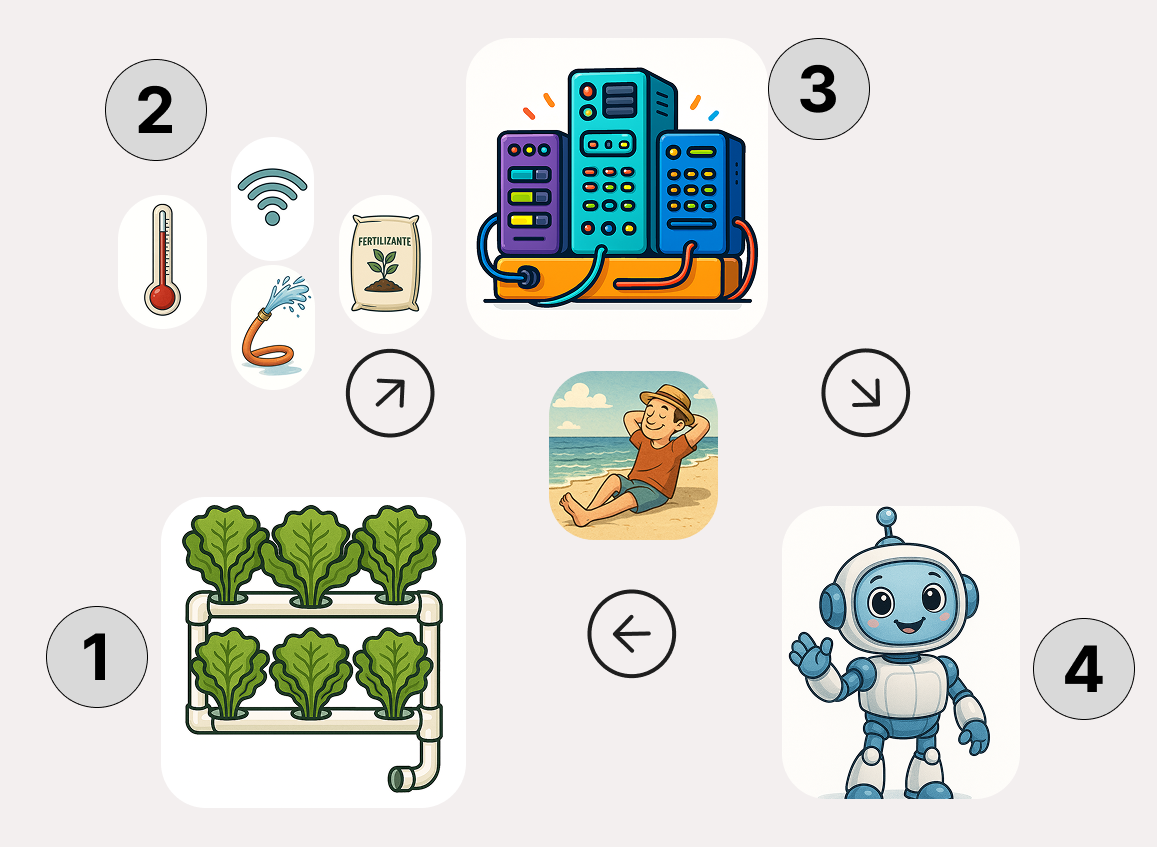
\includegraphics[scale=0.2]{Illustrations/Figura 3.png} % sem extensão se for .png
    \caption{Exemplo de funcionamento do sistema proposto}
    \label{fcht:figura3}
    % \SourceOrNote{Autoria Própria (2024)} % só se esse comando estiver definido
\end{figure}

Na etapa c) Definição das tecnologias, layout do sistema e funcionalidades, primeiramente foi escolhido o Figma (uma plataforma online e gratuita) para desenvolvimento do design e validação dos fluxos. Para o desenvolvimento da API (do inglês, Application Programming Interface, Interface de Programação de Aplicativos), responsável pela integração entre os sistemas e usuário, foi escolhido o Javascript (graças a compatibilidade com diversos dispositivos e vasto acervo de bibliotecas e frameworks) utilizando Node.js (ambiente de execução JavaScript de prototipagem rápida, integração natural com bancos de dados, demanda de poucos recursos de hardware e escalável), React (biblioteca JavaScript usada para criar interfaces de usuário baseada em atualizações rápidas, componentes reutilizáveis e muito utilizado em aplicações web) e armazenamento em banco de dados não-relacional MongoDB (gratuito, com esquema flexível para armazenagem de registros, com alta performance para leituras e escritas específicas e desenvolvimento ágil).
O layout do sistema foi projetado para ser o mais simples e intuitivo, facilitando o uso desde o usuário sem familiaridade com sistemas computadorizados até o usuário avançado. 
As funcionalidades foram desenhadas com foco no monitoramento e controle da fazenda vertical. Inclui gráficos e relatórios on-line em nível de hortaliça cultivada.

A última etapa ( d) prototipação) focou em desenvolver um protótipo de baixa fidelidade, validando assim o layout, usabilidade e garantindo que  sistemao para o usuário. Na sequencia, utilizando-se das tecnologias elencadas anteriormente, foi desenvolvido um protótipo de alta fidelidade, implementando um conjunto de funcionalidades para verificar a viabilidade técnica da API. Foi criado um servidor (back-end) Node.js para receber os dados simulados tanto do cliente quanto dos sensores e IA. O MondoDB foi configurado com uma coleção para armazenar os dados. Também foi criada uma interface  web (front-end) em React conectada ao back-end. As funcionalidades implementadas na interface foram uma tela de login (apenas usuários cadastrados podem acessar o sistema,  dashboard em tempo real (exibe os dados da fazenda vertical em tempo real), painéis laterais com informações atualizadas, campos para que o usuário possa alterar as informações, tela para cadastro de mais de uma fazenda vertical por usuário e também opção para que o usuário possa atualizar seus próprios dados.	

\section*{RESULTADOS PRELIMINARES}\label{sect:resultados}

Em desenvolvimento.

\section*{CONCLUSÃO}\label{sect:conclusao}

Em desenvolvimento.

\printbibliography

%% Elementos pós-textuais (opcionais): Apêndice e Anexo
%Caso for utilizar, basta retirar o símbolo de % na frente do comando
%%%%% Elementos pós-textuais
%%
%% Glossário, apêndices, anexos e índice remissivo (opcionais).

%% Apêndices
\begin{Appendix}

\section{Título de Apêndice}%
\label{sect:apx-a1}

Exemplo de apêndice (\Cref{sect:apx-a1}) em uma seção de \nameref{sect:appendix}.

\subsection{Título de Seção Secundária de Apêndice}%
\label{ssect:apx-a2}

Exemplo de seção secundária de apêndice (\Cref{ssect:apx-a2}).

\subsubsection{Título de Seção Terciária de Apêndice}%
\label{sssect:apx-a3}

Exemplo de seção terciária de apêndice (\Cref{sssect:apx-a3}).

\paragraph{Título de seção quaternária de Apêndice}%
\label{prgh:apx-a4}

Exemplo de seção quaternária de apêndice (\Cref{prgh:apx-a4}).

\subparagraph{Título de seção quinária de Apêndice}%
\label{sprgh:apx-a5}

Exemplo de seção quinária de apêndice (\Cref{sprgh:apx-a5}).

\end{Appendix}

%% Anexos
\begin{Annex}

\section{Título de Anexo}%
\label{sect:anx-a1}

Exemplo de anexo (\Cref{sect:anx-a1}) em uma seção de \nameref{sect:annex}.

\subsection{Título de Seção Secundária de Anexo}%
\label{ssect:anx-a2}

Exemplo de seção secundária de anexo (\Cref{ssect:anx-a2}).

\subsubsection{Título de Seção Terciária de Anexo}%
\label{sssect:anx-a3}

Exemplo de seção terciária de anexo (\Cref{sssect:anx-a3}).

\paragraph{Título de seção quaternária de Anexo}%
\label{prgh:anx-a4}

Exemplo de seção quaternária de anexo (\Cref{prgh:anx-a4}).

\subparagraph{Título de seção quinária de Anexo}%
\label{sprgh:anx-a5}

Exemplo de seção quinária de anexo (\Cref{sprgh:anx-a5}).

\end{Annex}

%% Índice remissivo
\printindex%


%% Fim do documento
\end{document}